\section{Background} \label{sec:background}

% (1 Page)

\begin{comment}
    Spectroscopy
    - What is spectroscopy
    - What is an emission line
    - What an emission line allows to know
    - Common patterns in spectroscopy

    Sparse Coding
    - Global definition
    - Signal Applications
    - Dictionary
    - Mathematical Formulation: Equation and parameters
    - Approx Resolution of the Formulation
    - Type of Dictionaries: Defined and Learned
    - Applications to Images and De-noising

    Link between Spectroscopy and Sparse Coding
    - Variability Factors in Spectroscopy
    - High Dimensionality and Co-linearity
    - Sparse Coding as solution
    - Tools used (package)
\end{comment}


% Spectroscopy
\subsection{Spectroscopy}
% What is spectroscopy
Spectroscopy is a technique that enables the analysis of interaction between matter and light \citep{smith_mr_sp_2005}.
This analysis provides information on chemical structures and physical forms that can be used to identify substances from the characteristic spectral patterns.
These patterns appear as light intensity peaks observed along the spectra, known as emission lines \citep{struve_fundamentals_1989}.
% What is an emission line
Each line has a different frequency depending on the molecule and energy level associated to it \citep{smith_mr_sp_2005}.

% What an emission line allows to know
Detection of emission lines and subsequent association with a molecule's isotope allow to know stellar objects's molecular structure.
The combination of emission lines for each object generates an unique fingerprint.
This allows to identify similar objects observing the similarities between observed spectra and theoretical known behavior of molecules \citep{howley_effect_2005}.

% Factors that make this problem non-trivial
A traditional process to identify lines consist on mapping observed frequencies to theoretical ones.
Unfortunately, observed and theoretical intensities do not coincide. For instance,
two spectral lines that are close in the frequency space are hard to dissociate, mainly because they appear
as lines with double peaks or blended into one single line \citep{cernicharo_detection_2013, smith_molecular_2015}.

% Common patterns in spectroscopy
Internal factors such as the temperature of objects, travel speed, type of astronomical object and its belonging to interstellar or intergalactic space \citep{sembach_far_2001} cause variability in the observed spectra.
However, the presence of lines within objects of similar composition are in general similar.
Lines present from the same isotope at different state energy levels, and thus, different frequencies, reinforces the hypothesis that an isotope is present.
This analysis of the presence and co-presence of spectral lines from the same isotope is known as rotational spectroscopy \citep{schilke_line_2001}.

There exists a relationships among intensity lines when homogeneous temperature and origin are assumed, i. e., local thermodynamic equilibrium (LTE) exists.
For different stellar objects, and for different spectra measured within the same object, intensities of spectral lines with the same frequency may vary \citep{madden_classification_2005}.
However, relationships between intensities of rotational sequences for the same object should be consistent but not necessarily linear \citep{nummelin_three-position_2000, smith_molecular_2015}, as can be seen in figure \ref{fig:spectral_lines}.

Noise and lack of sensitivity in the measurements can either modify the frequency of a spectral line or produce false positives \citep{nummelin_three-position_1998}.
This makes mandatory to involve astronomers to perform the identifications \citep{schilke_line_2001}.

\begin{figure}[H]
   	\begin{center}
   		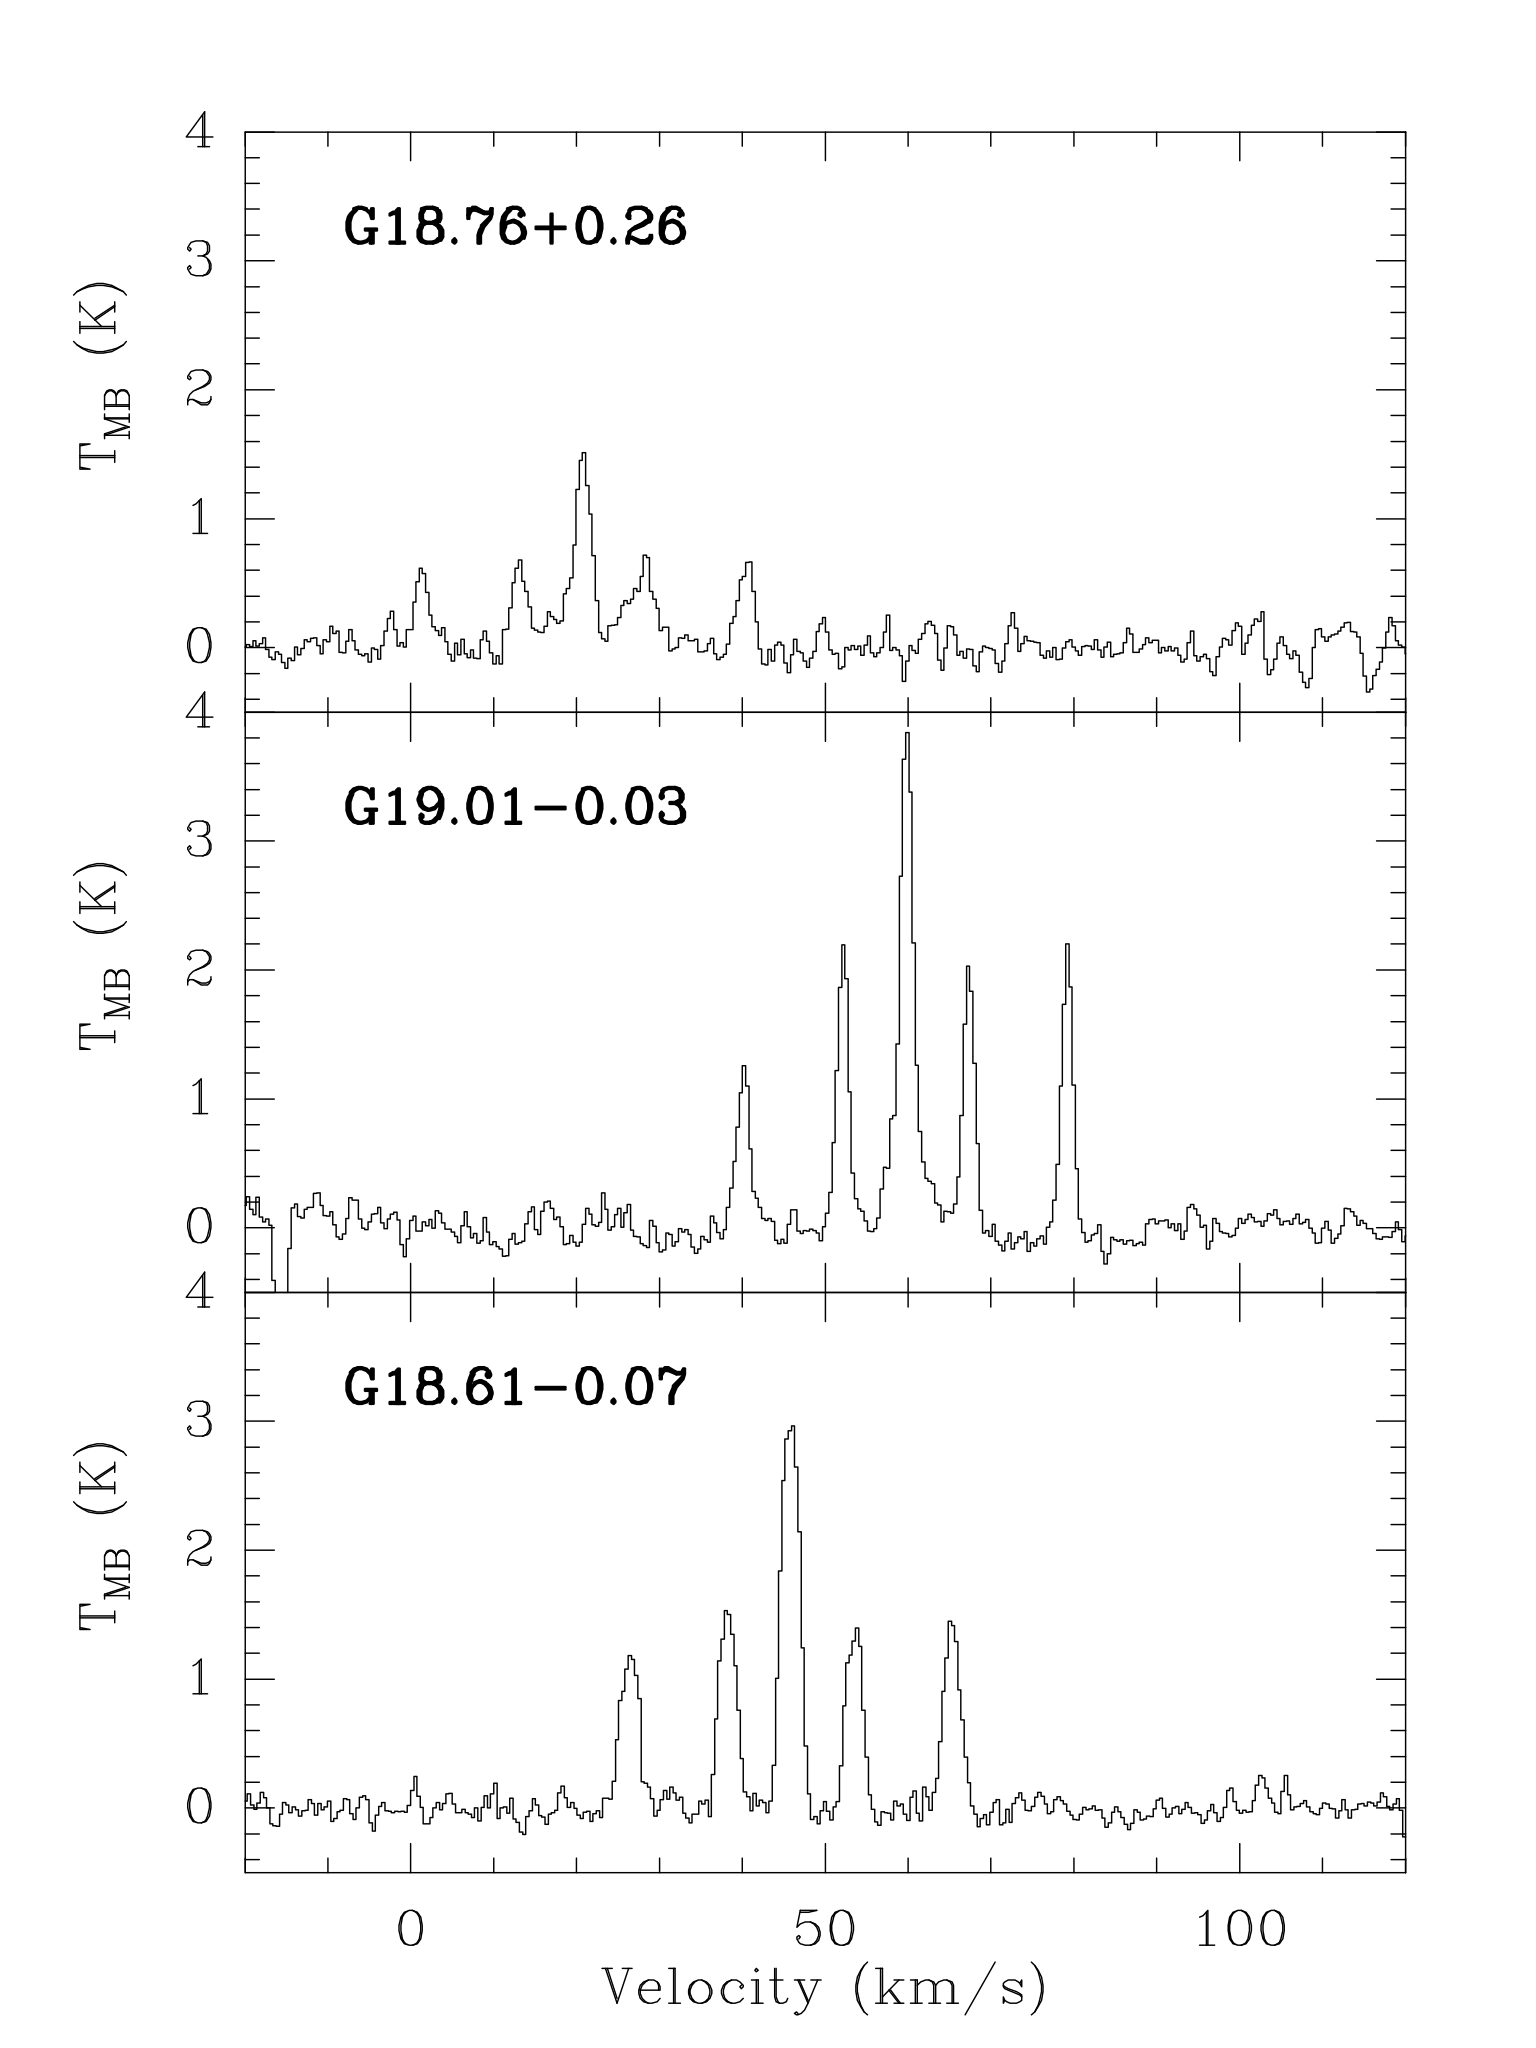
\includegraphics[width=0.40\textwidth]{images/spectral_lines}
   		\caption{Example spectra in a NH$_3$ transition for three sources.
   			We can see variations in velocity and intensity besides the similar structure \citep{schuller_atlasgal_2009}.}
   		\label{fig:spectral_lines}
   	\end{center}

\end{figure}

% Sparse Coding
\subsection{Sparse coding}
% Global Definition
Sparse coding consist in modelling signals through linear combinations of basis vectors under sparsity constraints,
in order to have a sparse representation of input signals \citep{mairal_online_2009, bristow_fast_2013}.
%
% Signal Applications
Sparse coding aims to represent or recover a signal through a reconstruction procedure.
We can divide this process in two main steps:
i) find a set of fundamental components able to represent any possible signal by linearly combining the components;
ii) for a given signal, determine the coefficients of the linear combination that minimize the difference between the signal and the linear combination of the components.
% Dictionary
Fundamental components set is known as \textit{dictionary}, where each component is called a \textit{word} \citep{mairal_online_2009}.
%
% Mathematical Formulation: Equation and parameters

Formally, let $s = [s_1, s_2, \ldots, s_n]$ be a given signal, where $s_i \in [0, 1] \; \forall i \in [1, \ldots, n]$.
Let $D = \{ w_1, w_2, \ldots, w_d \}$ be the dictionary, where $w_i = [w_{i1}, \ldots, w_{in} ]$ and $w_{ik} \in [0,1] \; \forall i \in [1, \ldots, d] \; \forall k \in [1, \ldots, n]$. Let $\alpha = [ \alpha_1, \ldots,  \alpha_d]$
be the set of coefficients such that $s = \sum_{i=1}^{d} \alpha_i \; w_i $.
Equation \ref{eq:sparse_coding} corresponds to the optimization problem that has to be solved in order to determine the sparse coding coefficients.

\begin{equation}
	\label{eq:sparse_coding}
    \begin{aligned}
		\text{Minimize}
		& _{\alpha} ||s- \sum_{i=1}^{d} \alpha_i \; w_i  ||_2^2  \\
		\text{Subject to: }
		& ||\alpha||_1 \leq \lambda \\
		& \alpha \geq 0 \\
	\end{aligned}
\end{equation}
where $||()||_k$ is the L-$k$ norm, and $\lambda$ is sparsity-inducing constant.

The solution to this problem is known as positive basis pursuit \citep{chen_atomic_2001} or positive lasso regression \citep{efron_least_2004}.
The optimization solution solved in closed form is very expensive in terms of processing \citep{mairal_online_2009}, instead,
we use the iterative algorithm presented in \citet{turlach_simultaneous_2005, mairal_optimization_2013}.

There are two constraints applied to alpha values: i) the lambda sparsity-inducing constraint allows the algorithm to select a convenient set of basis vectors so that the number of non-zero values minimized;  ii) the positive formulation of the problem allow us to give a meaningful use to the found set of alpha values; both are detailed in section \ref{sec:algorithm}. 

% Type of Dictionaries: Defined and Learned
In sparse coding, there exist two types of possible dictionaries to create the basis vector set:
i) Previously defined one, where a set is selected accord to the nature of signal domain.
ii) Automatically learned one, where methods such as clustering or another generalization searching are used \citep{mairal_online_2009}.
For wavelength domains, predefined dictionaries give satisfactory results \citep{mallat2009}.

% Applications to Images and De-noising
%Sparse Coding is a well known technique in visualization applications.
%Example of this are image classification, de-noising and image reconstruction \citep{mairal_online_2009}.
%In these cases, words are automatically learned as patches from image sets.
%Then, the most representatives patches are selected to replicate as much images as possible from the learned image sets.
% Tools used (package)
%The software used in this work is the Python library SPAMS available for Matlab and R as well \footnote{\url{http://spams-devel.gforge.inria.fr/}}. \citep{mairal_online_2009,mairal_online_2009_2}
